\documentclass[12pt,letterpaper,noanswers]{exam}
\usepackage[usenames,dvipsnames,svgnames,table]{xcolor}
\usepackage[margin=0.9in]{geometry}
\renewcommand{\familydefault}{\sfdefault}
\usepackage{multicol}
\pagestyle{head}
\header{AM 108 Class 19}{}{bifurcations}
\runningheadrule
\headrule
\usepackage{graphicx} % more modern
\usepackage{amsmath} 
\usepackage{amssymb} 
\usepackage{hyperref}
\usepackage{tcolorbox}

\begin{document}
 \pdfpageheight 11in 
  \pdfpagewidth 8.5in

\noindent 




\begin{itemize}

   
    \item If you have not completed it, fill out the project preference form (it is on Gradescope - upload it there when done).  In general, groups will be three people.  If there is currently one other person you'd prefer to work with, list them in your preferences.
    \item There will be a pre-class assignment for Monday.
    \item There will be a skill check in class on Monday.  The problem info is below.
 \item Problem set 08 is due Friday October 30th.
\end{itemize}

\hrule
\vspace{0.2cm}



\noindent\textbf{Teams}

\begin{multicols}{2}
1. 
\end{multicols}

\noindent \textbf{Teams 1 and 2}: Post screenshots of your work to the course Google Drive today.  Include words, labels, and other short notes that might make those solutions useful to you or your classmates.  Find the link in Canvas (or here: \url{https://drive.google.com/drive/u/0/folders/1GcpwvKHD4tMecpFQ4lNxN_r5Ylj7YHbd})

\vspace{0.2cm}

\hrule
\vspace{0.2cm}

\noindent\textbf{Polls}


\vspace{0.2cm}

\hrule
\vspace{0.2cm}

\noindent\textbf{Big picture}

We are looking at how bifurcations manifest in 2d systems.  The saddle-node, transcritical, and pitchfork bifurcations generalize from occuring when $f'(x^*) = 0$ to occurring when $\left.Df\right\vert_{\underline x^*}$ (the Jacobian matrix evaluated at the fixed point) has a zero eigenvalue.

We have some new bifurcations that can occur in 2d systems and don't exist in 1d systems.  The Hopf bifurcation is one of these and is a bifurcation in which a fixed point changes stability and a limit cycle is born/annihilated.  


\vspace{0.2cm}
\hrule
\vspace{0.2cm}

\noindent \textbf{Extra vocabulary / extra facts:}
\begin{tcolorbox}
A Hopf bifurcation in which a stable limit cycle is born is called \textbf{supercritical}.  When an unstable limit cycle is born the bifurcation is \textbf{subcritical}.  

A \textbf{subcritical Hopf} is associated with a jump, or even a catastrophic change, in the system state.
\end{tcolorbox}

subcritical Hopf:
\url{https://www.youtube.com/watch?v=zclp8vLKJzU}

oscillating reaction:
\url{https://www.youtube.com/watch?v=IggngxY3riU}

spatially extended oscillating reaction:
\url{https://www.youtube.com/watch?v=PpyKSRo8Iec}

\vspace{0.2cm}
\hrule
\vspace{0.2cm}


\noindent\textbf{Skill Check C20 practice}
\begin{questions}
\item Retake of skill check C17: setting up an integral for the time it takes to traverse a curve.


\item The plots below show the trace and determinant vs a parameter for two different fixed points that occur in a system.

Using the following graphs of the trace and determinant, classify the bifurcation(s),  identify the approximate bifurcation point(s), and identify the types of fixed points involved.

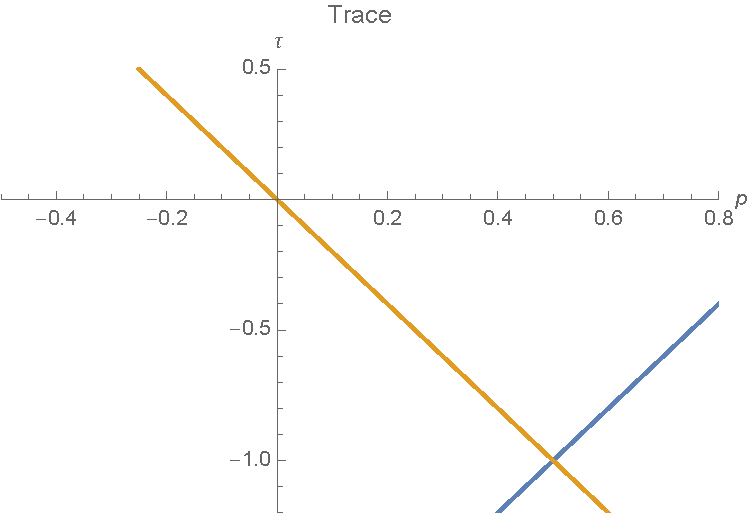
\includegraphics[width=0.4\linewidth]{img/C19-20p1a.pdf}
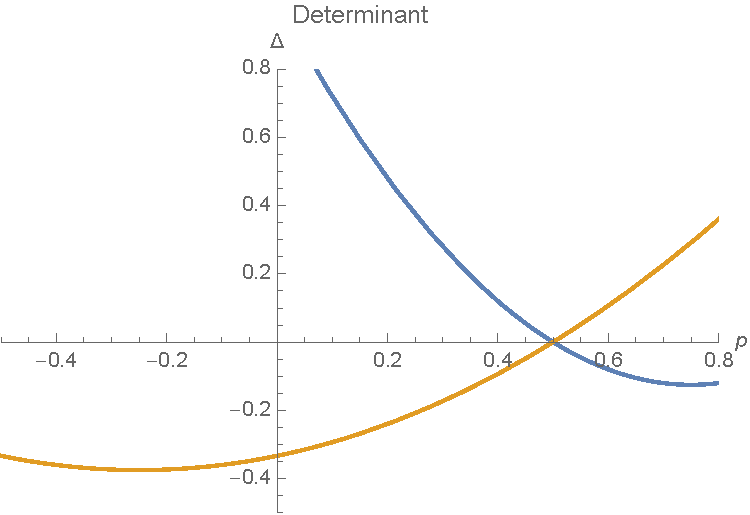
\includegraphics[width=0.4\linewidth]{img/C19-20p1b.pdf}

\end{questions}

\vspace{0.2cm}

\hrule
\vspace{0.2cm}

\noindent\textbf{Skill check C20 practice solution}

We are looking for parameter values when $\Delta = 0$ (for saddle-node, transcritical, pitchfork) or when $\tau = 0, \Delta>0$ (for Hopf).

The orange curve crosses $\Delta = 0$ at $p=0.5$.  When $p=0.5$, we have $\tau < 0$, so the orange fixed point transitions from a saddle point for $p<0.5$ to a stable fixed point for $p>0.5$.

The blue curve crosses $\Delta = 0$ at $p = 0.5$.  When $p=0.5$, we have $\tau<0$ so the blue fixed point transitions from stable to saddle as $p$ increases through $p=0.5$.

The orange curve crosses $\tau = 0$ at $p=0$, but $\Delta<0$, so it is not a bifurcation.

There is one bifurcation.  It involves a saddle point and a stable node exchanging stability, occurs at $p=0.5$, and is a transcritical bifurcation.

\vspace{0.2cm}

\hrule
\vspace{0.2cm}
\noindent\textbf{Questions}

\noindent \ \ 0.  What do you like to do for exercise? (and write your names on the slide).

\begin{questions}
\question (8.1.6) Consider the system
\begin{align*}
\dot{x} = &\ y - 2x \\
\dot{y} = &\ \mu+x^2-y.
\end{align*}
\begin{parts}
\item Sketch the nullclines.
\item Find and classify the bifurcations that occur as $\mu$ varies.
\item Show that at the point of bifurcation the $\dot{x}=0$ and $\dot{y}=0$ nullclines are tangent.  
\item Do you expect this to usually be true for a saddle-node bifurcation?  What about for a transcritical or pitchfork bifurcation?
\end{parts}

\question (8.2.8) Consider the dimensionless predator-prey system:
\begin{align*}
\dot{x} = &\ x(x(1-x)-y) \\
\dot{y} = &\ y(x-a), \quad a>0.
\end{align*}
\begin{parts}
\item Which variable is representing prey, and which predators?
\item Find the fixed points of this system. (You can use Mathematica or do this by hand)
\item Determine the stability of these fixed points.  (You can use Mathematica or do this by hand)  \emph{The trace and determinant will be sufficient to classify two of the points.  For the third fixed point, drawing the nullclines may help you classify it.  Note that your classification will include different cases for different ranges of $a$.}
\item Make a variation on a bifurcation diagram by showing the locations of the fixed points: plot the $x$ value associated with each fixed point vs $a$ for $0 < a < 2$.  Used dashed lines for unstable or saddle points and solid lines for stable points.
\item What type of bifurcation occurs when $a=1$?  What about when $a = \frac{1}{2}$?
\item Estimate the frequency of limit cycle oscillations for $a$ very close to the bifurcation.
\item Does the Hopf bifurcation appear to be supercritical or subcritical?  

To allow you to see the direction of forward time, the cyan curve corresponds to time $0$ to $50$ of a forward integration, and the black curve to time $50$ to $400$.  The $a$ value is given in the caption of each plot.

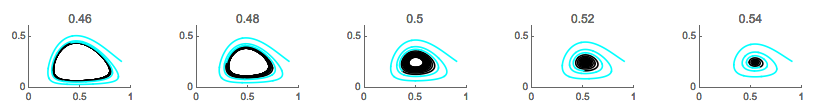
\includegraphics[width=6in]{img/S19C17p1.png}

\end{parts}


\question (8.6.1: ``Oscillator death'' and bifurcations on a torus)  We have worked with models of a single oscillator following a reference oscillator but haven't had the chance to work with a model where each oscillator responds to the other oscillator.

This model is from Ermentrout and Kopell (1990), where the authors were considering a system of interacting neural oscillators.  They developed a simple example with two interacting oscillators that captured many of the interaction properties they wanted for their neural system.  Specifically, they wanted to capture that coupling between oscillators can actually suppress oscillation (``oscillator death'') and lead to a steady state of the coupled system.  Here is their example model:
\begin{align*}
\dot{\theta_1} = &\ \omega_1 + \sin \theta_1 \cos\theta_2 \\
\dot{\theta_2} = &\ \omega_2 + \sin \theta_2 \cos\theta_1.
\end{align*}
The oscillators have a natural frequency, but they also are responding to each other.

There are a number of different behaviors possible in this system.
We will work to figure out the possible behaviors by identifying bifurcations and  plotting a stability diagram in $\omega_1\omega_2$ space.

\begin{parts}
\item Looking for fixed points of $\phi = \theta_1-\theta_2$ allows us to identify curves where $\theta_1 = \theta_2 + c$ where $c$ is a constant. 

Here, use both $\phi = \theta_1 - \theta_2$ (``phi'') and $\psi = \theta_1 + \theta_2$ (``psi'') to aid your analysis.  

If $\dot{\phi} = 0$ and $\dot{\psi} = 0$ (and only if this is true) then the system has a fixed point.  Why is that?
\item Find $\dot{\phi}$ and $\dot{\psi}$ equations.  \emph{Look up trig identities as needed.}
\item In what region of the $\omega_1\omega_2$ plane does the system have fixed points?
\item In what regions of the $\omega_1\omega_2$ plane does this system have $\dot{\phi} = 0$ or $\dot{\psi} = 0$ but not both?  Sketch a phase portrait in the $\theta_1\theta_2$ plane in such a case.
\end{parts} 

\end{questions}

\eject

1: a: The $\dot{x} = 0$ nullcline is in black and the $\dot{y} = 0$ nullcline is in blue for three different values of $\mu$.  These values
are below, at, and above the bifurcation point.


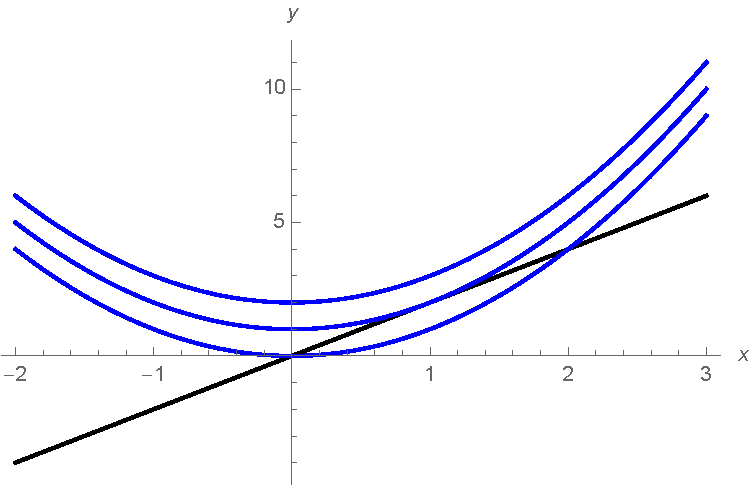
\includegraphics[width=2.5in]{img/C15nullclines.pdf}


b: To find and classify the bifurcations we need to identify the fixed points and find where the number of fixed points changes.
We can see from the nullclines that the black and blue lines intersect in two places for some values of $\mu$, and as $\mu$ increases
they intersect at a single point and then no points.  This means there's a saddle-node bifurcation.  So I've classified the bifurcation just
from looking at the nullcline picture.  To find the bifurcation, I suppose I need to find the point where there's just one fixed point, or, I can
find one of the fixed points and identify where it changes stability.  Either option would work.

At the fixed points $y = 2x$ and $y = \mu + x^2$ because $y-2x = 0$ and $\mu + x^2 - y = 0$.
This means $2x = \mu + x^2$ so $x^2 - 2x + \mu = 0$.  Using the quadratic formula,
\[x_\pm = 1 \pm \frac{1}{2} \sqrt{4 - 4\mu} = 1\pm \sqrt{1 - \mu}.\]
So there is just a single fixed point when $\mu = 1$ and for $\mu >1$ there are no fixed points.  Thus the bifurcation occurs
when $\mu = 1$ % at the point $(1, 2)$.

c: The slope of the $\dot{x} = 0$ nullcline of $y = 2x$ is $2$.  We want to show the other nullcline has the same slope at the point
of bifurcation.  The other nullcline is $y = x^2 + \mu$ so its slope is given by $2x$ and at the bifurcation point, $x = 1$, so its slope is also 2.
The two lines intersect at $(1,2)$ for $\mu = 1$ and they have the same slope, so they are tangent.

d: Assume we have two nullclines that are continuous and differentiable.  At the bifurcation, they need to intersect in a single point, while just before (or just after) the bifurcation they need to intersect in multiple nearby points.  I'm assuming the nullclines are smooth curves (without sharp corners), so the nullclines will be tangent at the bifurcation.

2: prey: $x$, predator: $y$.  fixed points: $(0,0)$, $(1,0)$, and $(a,a-a^2)$.  classification: $(0,0)$ a saddle for $a>0$, $(1,0)$ a saddle for $0<a<1$, stable for $a>1$.  $(a,a-a^2)$ unstable for $0<a<\frac{1}{2}$, stable for $\frac{1}{2}<a<1$ and a saddle for $a>1$.  Hopf at $a_c = 1/2$.   At $a_c = 1$ two fixed points exchange stability (and collide) so transcritical.  frequency of oscillation is given by the imaginary part of the eigenvalues near $a_c$ so $\omega \approx \frac{1}{2\sqrt{2}}$. Stable limit cycle at $a = 0.46, 0.48$ and stable spiral at $0.52,0.54$ so appears to be supercritical.


3a: Assume $\dot \phi = 0$ and $\dot \psi = 0$.  Then $\dot \phi + \dot \psi = 2\dot \theta_1 = 0$ so $\theta_1$ is fixed and $\dot \psi - \dot\phi = 2\theta_2 = 0$ so $\theta_2$ is fixed.  Going the other direction, if $\dot\theta_1 = 0$ and $\dot\theta_2=0$ then their sum and their difference is zero as well.

3b: $\dot\phi = \omega_1 - \omega_2 + \sin\theta_1\cos\theta_2 - \sin\theta_2\cos\theta_1 = \omega_1-\omega_2 + \sin(\theta_1 - \theta_2) = \omega_1-\omega_2 + \sin(\phi).$

$\dot\psi = \omega_1 + \omega_2 + \sin\theta_1\cos\theta_2 + \sin\theta_2\cos\theta_1 = \omega_1+\omega_2 + \sin(\theta_1 + \theta_2) = \omega_1+\omega_2 + \sin(\psi).$

3c: fixed points when $\dot \phi = 0$ and $\dot\psi = 0$ so need $\vert\omega_1 - \omega 2\vert\leq 1$ and $\vert \omega_1+\omega_2 \leq 1$.  Draw the lines $\omega_1 -\omega_2 = 1$, $\omega_1-\omega_2 = -1$, $\omega_1+\omega_2 = 1$ and $\omega_1+\omega_2 =-1$.  These lines enclose a square region (tilted 45 degrees) centered around the origin where there are fixed points.

3d: $\dot\phi = 0$ but $\dot\psi$ happens for $-1\leq \omega_1 - \omega_2 \leq 1$ and $\omega_1+\omega_2 >1$ or $\omega_1+\omega_2 < -1$.  The region between the orange and green lines below is a region where one is zero but not both.  In the $\omega_1\omega_2$ plane there are four such regions.

Assume $\dot\phi = 0$. The systems are completely decoupled, so we can just think about the $\phi$ system.  There exists a steady state $\phi$ value, $\phi_s = c$ (and usually two: one stable and one unstable).  These correspond to a steady state relationship $\theta_1 = \theta_2 + c$.  So there are two closed orbits...


\end{document}